%%%%%%%%%%%%%%%%%%%%%%%%%%%%%%%%%%%%%%%%%%%%%%%%%%%%%%%%%%%%%%%%%%%%%%%%%%%%%%
%   Sample paper (in LaTeX2e) for Annales Univ. Sci. Budapest., Sect. Comp.  %
%                                                                            %
%                       http://ac.inf.elte.hu                                %
%                                                                            %
%%%%%%%%%%%%%%%%%%%%%%%%%%%%%%%%%%%%%%%%%%%%%%%%%%%%%%%%%%%%%%%%%%%%%%%%%%%%%%




%%%%%%%%%%%%%%%%%%%%%%%%%%%%%%%%%%%%%%%%%%%%%%%%%%%%%%%%%%%%%%%%%%%%%%%%%%%%%%
%%%%%%%%%%%%%%%%%%%%%%%%%%%%%%%%%%%%%%%%%%%%%%%%%%%%%%%%%%%%%%%%%%%%%%%%%%%%%%
%%                                                                          %%
%%                             IMPORTANT:                                   %%
%%                  In case of any problems contact                         %%
%%                        ac@compalg.inf.elte.hu                            %%
%%                                                                          %%
%%%%%%%%%%%%%%%%%%%%%%%%%%%%%%%%%%%%%%%%%%%%%%%%%%%%%%%%%%%%%%%%%%%%%%%%%%%%%%
%%%%%%%%%%%%%%%%%%%%%%%%%%%%%%%%%%%%%%%%%%%%%%%%%%%%%%%%%%%%%%%%%%%%%%%%%%%%%%


\documentclass[10pt,leqno,twoside]{article}
\usepackage{graphicx}
\usepackage{annal-latex}
\usepackage{makeidx,latexsym,amssymb}
%%%%%%%%%%%%%%%%%%%%%%%%%%%%%%%%%%%%%%%%%%%%%%%%%%%%%%%%%%%%%%%%%%%%%%%%%%%%%%%%%%%%%%%%%%%%%%%
%%%% Your numbering system for theorems etc. may be different from the one suggested below. %%%
%%%%%%%%%%%%%%%%%%%%%%%%%%%%%%%%%%%%%%%%%%%%%%%%%%%%%%%%%%%%%%%%%%%%%%%%%%%%%%%%%%%%%%%%%%%%%%%


\newtheorem{theorem}{\indent Theorem}[section]
\newtheorem{proposition}[theorem]{\indent Proposition}
%\newtheorem{lemma}[theorem]{\indent Lemma}
\newtheorem{lemma}{\indent Lemma}[section]
\newtheorem{corollary}{\indent Corollary}[section]


%\theoremstyle{definition}
%\newtheorem{definition}[theorem]{\indent Definition}
\newtheorem{definition}{\indent Definition}[section]
\newtheorem{example}[theorem]{\indent Example}
\newtheorem{remark}{\indent Remark}[section]



%%% An unnumbered object: %%%
\newtheorem*{xrem}{\indent Remark}


\begin{document}
\setcounter{page}{1}
\newcommand\balline{\small Vu L. A. et al.}
\newcommand\jobbline{\small Evaluate scientific publications by N-linear ranking model}

\vspace{-4cm} \fofej{42}{14}{nn}{nnn}

\vspace{.4cm}

\title{Evaluate scientific publications by N-linear ranking model}

\author{{\bf Vu Le Anh} (Ho Chi Minh city, Vietnam)\\[1ex]
{\bf Hai Vo Hoang} (Ho Chi Minh city, Vietnam)\\[1ex]
{\bf Hieu Le Trung} (Da Nang, Vietnam)\\[1ex]
{\bf Kien Le Trung} (Thua Thien Hue, Vietnam)\\[1ex]
{\bf Jason J. Jung}(Gyeongsan, Korea)}
%% More authors can be given by repeting the \author comand)


%
\keywords{N-star ranking, Markov chain, PageRank, Academic ranking, Conference ranking, Ranking algorithms, Prolific ranking, Recommendation systems, Bibliographical database, DBLP}
%
\mathclass{Please use the \textit{2010 Mathematics Subject Classification}}
%

\projsupport{This work is the extend version of the paper "A General Model for Mutual Ranking Systems" in \textit{Intelligent Information and Database Systems
Lecture Notes in Computer Science} \textbf{Volume 8397}, 2014, pp 211-220 }
%

%\begin{center}
%\textit{Dedicated to ...}
%\end{center}


%%%%%%%
% We shall fill out "???"
%%%%%%%%

\commby{???}
\vspace{-2ex}
\recacc{???}{???}

\vspace{-7ex}

\abstract{
Ranking has been applied in many domains using recommendation systems such as search engine, e-commerce, and so on.
We will introduce and study N-linear mutual ranking, which can rank $n$ classes of objects at once. The ranking scores of these classes are dependent to the others. For instance, PageRank by Google is a 2-linear ranking model, which ranks the web-pages and links at once.
Particularly, we focus to $N$-star ranking model and demonstrate it in ranking conference and journal problems. We have conducted the experiments for our models versus classical ones. The experiments are based on the DBLP dataset, which contains more than one million papers, authors and thousands of conferences and journals in computer science. The experimental results show that $N$-star ranking model evaluates everything much more detail based on the context of their relationships.
}
\section{Introduction}
Ranking is an interesting but difficult problem on many information processing systems. With a large amount of information, the systems need to adapt efficient ranking schemes to sort out (or to select) only the information which are highly relevant to the users' contexts.
Particularly, in the context of \emph{bibliometrics}, % a reference?
a set of given entities can be quantified to compare several evaluation indicators (e.g., popularity and reputation). For example, impact factors (IF) of international journals can be measured by taking into account how many times the papers in the corresponding journals have been cited.

In this work we focus on a system of ranking classes. Their ranking scores have mutual dependencies, which can expressed by a system of linear equations. Let us explain the ideas by two examples.

\textit{PageRank}. PageRank is very well-known ranking for website \cite{pagerank98}, which were applied in Google search engine. We rewrite the original formula by a system of two generic linear equations describing the mutual dependency of ranking of two classes, $Web$ and $Link$.
{\small
\begin{equation}\label{eq:PR1}
Link ~\longleftarrow~ 100\% \times Web
\end{equation}
\begin{equation}\label{eq:PR2}
Web ~\longleftarrow~ 85\% \times Link + 15\%\times Random
\end{equation}
}

Equation \ref{eq:PR1} says that the rank score of a link is determined by the rank score, which is the link from. Equation \ref{eq:PR2} says that the rank score of a web is determined  by 85\% from the rank score of links, which refers to the web; and 15\% from randomness. Thus the rank scores of webs and links are mutual dependent. Moreover, we prove that there exists only one rank scores satisfy the above system of linear equations.

\textit{Ranking scientific publication}. We propose a model for ranking 4 classes Authors ($Author$), Publications ($Pub$), Conference ($Conf$) and Citations ($Cite$). Their relationships are described by following a system of four generic linear equations.
{\small
\begin{equation}\label{eq:Pub1}
Author ~\longleftarrow~ 100\% \times Pub
\end{equation}
\begin{equation}\label{eq:Pub2}
Conf ~\longleftarrow~ 100\% \times Pub
\end{equation}
\begin{equation}\label{eq:Pub3}
Cite ~\longleftarrow~ 100\% \times Pub
\end{equation}
\begin{equation}\label{eq:Pub4}
\begin{split}
Pub ~\longleftarrow~ &30\% \times Author +  30\% \times Conf\\ 
&\qquad +  30\% \times Cite+  10\% \times Random
\end{split}
\end{equation}
}

Equation \ref{eq:Pub1} says that the rank score of each author is determined by the rank scores of his publications. Equation \ref{eq:Pub2} says that the rank score of each conference is determined by the rank scores of it publications. Equation \ref{eq:Pub3} says that the rank score of each citation is determined by the rank score of the publication, which is the owner of the citation. Equation \ref{eq:Pub4} says that the rank score of each publication is determined by 30\% from the rank score of its authors; 30\% from the rank score of its conference; 30\% from the rank scores of the cited-to citations; and 10\% from randomness.

Both of above ranking systems are described by systems of linear equations called \textit{N-linear ranking models}. Here are the key questions: \textit{Does the system of linear equations have a unique solution? How can we compute the solution?} And \textit{how do the models work in realistic ranking systems?} We solve only a part of problems by studying a special case of N-linear ranking model, \textit{N-star ranking model}. Both of two examples are N-star ranking models  and there exists unique solutions. Moreover we can estimate it by a loop of computing the linear function.


The main contribution and outline of this paper are as follows.

\textit{N-linear ranking model}. We describe the background of the  N-linear ranking model (Section \ref{Sect:Backgrounds}). N-linear ranking model is the system of $N$ ranking scores of $N$ classes. The rank scores are depend on others by a linear constraint system (Subsection \ref{Sect:N-linear}). We introduce the affect and reflect relation between classes (Subsection \ref{Sect:N-linear}). We explain these definitions in detail by the case study of PageRank (Subsection \ref{Sect:PageRank}).

\textit{N-star ranking model.} We define the N-star ranking model as a N-linear ranking model in which there exists a core class (Section \ref{Sect:N-star}). We prove that there exists unique N-star ranking model which satisfy  a given linear constraint system (Proposition \ref{prop:Existence}). We show that PageRank is a 2-star ranking model (Proposition \ref{prop:PR}). Finally, we describe the algorithm to compute scores of classes based on the linear constraint system.

\textit{Ranking bibliographical database}. We study two N-star ranking models for the author, publication and conference ranking problem in different contexts (Section 4).
The first model is general N-star ranking model for 4 classes: authors, publications, conferences, citations (Definition\ref{Def:4starGen}).
In the second model, we simplify the conditions by the assumption that everything is equal (Definition \ref{Def:4starSimple}).

\textit{Experiments}. We do the experiments for the simple  N-linear ranking model of authors, publications and conference ranking  (Section \ref{Sect:Experiments}). We have designed the three different datasets to adapt the limit of  computing resources (Subsection \ref{Sect:Dataset}). The datasets are classified into two contexts: with/ without citations.
We propose the models and the measurements for comparing different ranking scores in both contexts (Subsection \ref{Sect:Measure}). We show the results and have discussions over datasets (Subsection \ref{Sect:Result}).
Our results are quite different from the naive one's and provide us some interesting things.

\textit{Related works and conclusion}. We discuss the related works of N-linear ranking model (Section \ref{Sect:Related}).
We discuss the power and applicable ability of  N-linear ranking model (Section \ref{Sect:Conclusion}).




%%%%%%%%%%%%%%%%%%%%%%%%%%%%%%%%%%%%%%%%%%%%%%%%%%%%%%%%%%%%%%%%%%%%%%%%%%%%%%%%%%%%%%%%%%%%%%%%%%%%%%%%%%%%%%%%%%%%%%%%%%%%%%%%%%%%%%%%%%%%%%%%%%%%%%%%%%%%%%%%
\section{Backgrounds}\label{Sect:Backgrounds}\label{Sect:Background}
\subsection{N-linear mutual ranking system}\label{Sect:N-linear}
The couple $(\mathcal{A},R)$ is called a \emph{ranking system} if (i) $\mathcal{A} = \{a_1,\ldots,a_n\}$ is a finite set, and (ii) $R: \mathcal{A} \rightarrow [0;+\infty)$. $\mathcal{A}$ is called a \emph{class}, $a\in\mathcal{A}$ is called an \emph{object of the class} $\mathcal{A}$, and $R$ is called a \emph{score} of $\mathcal{A}$. $R$ is \emph{positive} if $R(a)>0 ~~\forall a \in \mathcal{A}$. $n = |\mathcal{A}|$ is the \emph{size} of $\mathcal{A}$.
\setlength{\parskip}{3pt}
\begin{definition}
$\Omega = \{(\mathcal{A}_i,R_i)\}_{i=1}^N$ is called a \emph{$N$-linear mutual ranking system} described by a system $\{\alpha_{ij},\beta_i,I_i,W_{ij}\}$ if $(\mathcal{A}_i,R_i)$ is a ranking system and $\alpha_{ij}, \beta_i \in [0;+\infty)$, $I_i=(t^{\texttt{\tiny(i)}}_u)_{n_i}$, $n_i = |\mathcal{A}_i|$, is a $n_i$-dimensional normalized nonnegative real number vector , $W_{ij}=(\omega^{\texttt{\tiny(ij)}}_{kl})_{n_i \times n_j}$ is a nonnegative real number and normalized columns matrix such that for all $i = 1,\ldots,N,$
\[\sum_j\alpha_{ij}+ \beta_i=1\qquad and \qquad R_i = \sum^N_{j=1}\alpha_{ij}W_{ij}R_j + \beta_i I_i.\]
\end{definition}
$\{\alpha_{ij},\beta_i,I_i,W_{ij}\}$ is called a \emph{linear constraint system} of $\Omega$.

Note that, generally since $\sum_i\alpha_{ij} + \frac{1}{N}\sum_j{\beta_j}$ is different one, a $N$-linear mutual ranking system is not a Markov chain. Let $a_{iu}, a_{jv}$ be objects in $\mathcal{A}_i, \mathcal{A}_j$ respectively. Suppose $\mathcal{C}^*(a_{iu},a_{jv})=\alpha_{ij}\omega^{\texttt{\tiny(ij)}}_{uv}.$
From the definitions, we have:
\[ R_i(a_{iu}) = \sum^N_{j=1}\sum^{n_j}_{v=1}\alpha_{ij}\omega^{\texttt{\tiny(ij)}}_{uv}R_j(a_{jv}) + \beta_i t^{\texttt{\tiny(i)}}_u=\sum^N_{j=1}\sum^{n_j}_{v=1}\mathcal{C}^*(a_{iu},a_{jv})R_j(a_{jv}) + \beta_i t^{\texttt{\tiny(i)}}_u\]
$a_{jv}$ is called \emph{affect to}  $a_{iu}$ (denoted by $a_{jv}\rightarrow a_{iu}$) if $\mathcal{C}^*(a_{iu},a_{jv})>0$. Class $\mathcal{A}_i$ is called  \emph{total affect and reflect directly to} class $\mathcal{A}_j$ (denoted by $\mathcal{A}_i\rightarrow \mathcal{A}_j$) if $\forall a_{jv}\in\mathcal{A}_j$:  $\exists a_{iu_1}, a_{iu_2}\in\mathcal{A}_i$: $a_{jv}\rightarrow a_{iu_2} \wedge a_{iu_1}\rightarrow a_{jv}$.
\begin{definition}
Class $\mathcal{A}_i$ is called  \emph{total affect and reflect to} class $\mathcal{A}_j$, denoted by $\mathcal{A}_i \rightsquigarrow \mathcal{A}_j$, if $\mathcal{A}_i\rightarrow \mathcal{A}_j$ or $\exists \mathcal{A}_k: \mathcal{A}_i\rightarrow \mathcal{A}_k \wedge \mathcal{A}_k \rightsquigarrow \mathcal{A}_j$.
\end{definition}

\subsection{PageRank}\label{Sect:PageRank}
We rewrite the PageRank into a 2-linear mutual ranking system as follows:

$\mathcal{W}= \mathcal{A}_1$ is the class representing for the set of webpages. $\mathcal{L}= \mathcal{A}_2$ is the class representing for hyperlinks. For each hyperlink $l\in \mathcal{L}$ from web $u\in \mathcal{W}$ to web $v \in \mathcal{W}$, we denote $u=in(l)$ and $v=out(l)$. For each $v \in \mathcal{W}$, we denote: $IN(v)=\{l \in \mathcal{L}|  v=out(l)\}$ and $N_{out}(v)=|\{ l\in \mathcal{L}| v=in(l)\}|$.
\setlength{\parskip}{3pt}

PageRank\cite{pagerank98} determined the ranking system of webpages by the following formula: $\forall v\in\mathcal{W}$,
\begin{equation}\label{eq01}
R_w(v) = d\sum_{l \in IN(v), u=in(l)} \frac{R_w(u)}{N_{out}(u)} + \frac{1-d}{|\mathcal{W}|}
\end{equation}
where $d\in (0,1)$ is a constant.
\setlength{\parskip}{3pt}

Suppose  $W_{21} = (\delta_{kt}) _{|\mathcal{L}|\times |\mathcal{W}|}$ is a matrix in which $\delta_{kt} = \frac{1}{N_{out}(w_t)}$ if $l_k\in \{l:~w_t = in(l)\}$, otherwise 0. $W_{21}$ is a nonnegative real number and normalized columns matrix. Suppose  $W_{12} = (\gamma_{tk}) _{|\mathcal{W}|\times |\mathcal{L}|}$ is a matrix in which $\gamma_{tk} = 1$ if $w_t= out (l_k)$, otherwise 0. We construct a 2-linear mutual ranking system on two classes $\mathcal{W}$ and $\mathcal{L}$ as follows: Let $\bar{R}_w$ and $\bar{R}_l$ be scores on the classes $\mathcal{W}$, $\mathcal{L}$ respectively. They are satisfied:
\begin{equation}\label{eq02}
\bar{R}_l = W_{21}\bar{R}_w\qquad and \qquad
\bar{R}_w = dW_{12}\bar{R}_l + (1-d)I_{|\mathcal{W}|},
\end{equation}
where $I_{|\mathcal{W}|}$ denotes the $|\mathcal{W}|$-dimensional vector in which all its elements are $1/|\mathcal{W}|$. It is not difficult to see that (\ref{eq02}) confirms: for all web $v\in\mathcal{W}$,
\[\bar{R}_w(v) = d\sum_{l \in IN(v), u=in(l)} \frac{\bar{R}_w(u)}{N_{out}(u)} + \frac{1-d}{|\mathcal{W}|}.\]

Since the equation (\ref{eq01}) has the unique solution which is the PageRank score (see in \cite{pagerank98}), $\bar{R}_w$ is the PageRank score $R_w$. Vice versa, if $R_w$ is a solution of (\ref{eq02}), $R_w$ should be $\bar{R}_w$. Thus, the PageRank score $R_w$ is totally determined by the equation (\ref{eq02}), or in other words, PageRank can be presented as the two-linear ranking system described by (\ref{eq02}).
\setlength{\parskip}{3pt}

Note that, since for each link $l\in \mathcal{L}$, let $u=in(l)$ and $v=out(l)$ then web $u$ affects to link $l$, ($u\rightarrow l$) and link $l$ affects to web $v$, ($l\rightarrow v$). Therefore, the class $\mathcal{W}$ total affect and reflect directly to the class $\mathcal{L}$, $\mathcal{W} \rightsquigarrow \mathcal{L}$.


%%%%%%%%%%%%%%%%%%%%%%%%%%%%%%%%%%%%%%%%%%%%%%%%%%%%%%%%%%%%%%%%%%%%%%%%%%%%%%%%%%%%%%%%%%%%%%%%%%%%%%%%%%%%%%%%%%%%%%%%%%%%%%%%%%%%%%%%%%%%%%%%%%%%%%%%%%%%%%%%
\section{N-star Ranking Model}\label{Sect:N-star}

\begin{definition}
Let $\Omega = \{(\mathcal{A}_i,R_i)\}^N_{i=1}$ be a $N$-linear mutual ranking system. $\Omega$ is called a $N$-\emph{star ranking} if
\begin{enumerate}
\item $\exists i :~ \mathcal{A}_i: (\beta_i >0)~\wedge$ $(I_i$ is positive $)\wedge (\forall \mathcal{A}_j(j\neq i): \mathcal{A}_i\rightsquigarrow\mathcal{A}_j$).
\item $\forall j\neq i :~ \alpha_{j1} = 1.$
\end{enumerate}
$\mathcal{A}_i$ is called a \emph{core} of the system $\Omega$.
\end{definition}

If $\Omega = \{(\mathcal{A}_i,R_i)\}^N_{i=1}$ is a $N$-star ranking system described by a linear constraint system $\{\alpha_{ij},\beta_{i},I_i,W_{ij}\}$, $\{\alpha_{ij},\beta_{i},I_i,W_{ij}\}$ is called $N$-\emph{star constraint system} of $\Omega$.

\begin{proposition}\label{prop:PR}
PageRank is a 2-star ranking system.
\end{proposition}
\begin{proof}
Because $1-d > 0$ and $\mathcal{W} \rightsquigarrow \mathcal{L}$, $\mathcal{W}$ is the core of PageRank. The second condition is clear since $\alpha_{21} = 1$. Hence, PageRank is a 2-star ranking system.
\end{proof}
The  ranking scores  are determined by  the $N$-star constraint system and the classes.
\begin{proposition}\label{prop:Existence}
Suppose the classes $\{\mathcal{A}_i\}^N_{i=1}$ and the $N$-star constraint system $\{\alpha_{ij}, \beta_{i},$ $I_i, W_{ij}\}$  are given. There exists a unique $\{R_i\}^N_{i=1}$ in which $R_i$ is a score on $\mathcal{A}_i$, such that $\Omega = \{(\mathcal{A}_i,R_i)\}^N_{i=1}$ is a $N$-star ranking described by $\{\alpha_{ij},\beta_{i},I_i,W_{ij}\}$ and for all $i$, $\sum_{a\in \mathcal{A}_i }R_i(a)=1$.
\end{proposition}
\begin{proof}
Assuming without loss of generality that $\mathcal{A}_1$ is a core of a $N$-star ranking system described by $\{\alpha_{ij},\beta_{i},I_i,W_{ij}\}$, the sequence of scores $R_1,\ldots,R_N$ satisfy the following equations:
\begin{equation}\label{eq03}
R_1 = WR_1 \qquad ~and~ \qquad
R_i = W_{i1}R_1 \qquad \forall i = 2,\ldots,N,
\end{equation}
where
\begin{equation}\label{eq39}
W = \alpha_{11}W_{11} + \alpha_{12}W_{12}W_{21} + \cdots + \alpha_{1N}W_{1N}W_{N1} + \beta_{1}{\bf I}_1
\end{equation}
and ${\bf I}_1$ is the $(n_1\times n_1)$-matrix which its columns are $I_1$. It is not difficult to infer that because $W_{1i}$ and $W_{i1}$ are transition matrices (i.e. nonnegative and normalized columns matrices), the new square matrix $W_{1i}W_{i1}$ is a stochastic matrix (i.e. a transition and square matrix). The matrices $W_{11}$ and ${\bf I}_1$ are also stochastic matrices. Since ${\bf I}_1$ has positive entries, $\beta_1 > 0$ (because $\mathcal{A}_1$ is the core), and $\sum_j\alpha_{1j} + \beta_1 = 1$, the matrix $W$ is also a stochastic matrix with positive entries. The Perron-Frobenius theorem (see in \cite{Keener1993,Kien09}) confirms that there exists a unique score $R_1$ with $\sum_{a\in\mathcal{A}_1}R_1(a) = 1$ such that
\[R_1 = WR_1.\]
From (\ref{eq03}), the unique existence of $R_1$ infers the unique existences of $R_2,\ldots,R_N$. Moreover, since $W_{21}, \ldots,W_{N1}$ are normalized columns and $\sum_{a\in\mathcal{A}_1}R_1(a) = 1$, we have $\sum_{a\in\mathcal{A}_i}R_i(a) = 1$ for all $i = 2,\ldots,N$. The proposition is proven.
\end{proof}
The ranking scores are computed by following algorithm:\\
\line(1,0){280}
~\\
{\bf Algorithm :} Finding the sequence scores $\{R_i\}^N_{i=1}$
~\\[-2mm]
\line(1,0){280}\\
\vspace{2mm}\enskip\enskip\textbf{Input :} $\alpha_{ij},~\beta_i,~W_{ij},I_i$\\
\vspace{2mm}\enskip\enskip\textbf{Output :} $\{R_i\}^N_{i=1}$\\
\textbf{{\scriptsize 1.}~~begin}\\
\textbf{{\scriptsize 2.}~~}~~~~~~Check the $N$-star ranking model with the core $\mathcal{A}_1$\\
\textbf{{\scriptsize 3.}~~}~~~~~~Let\\[-7mm]
\[W \leftarrow \alpha_{11}W_{11} + \sum^N_{i=2}\alpha_{1i}W_{1i}W_{i1} + \beta_1{\bf I}_1\qquad\qquad\qquad\]
\textbf{{\scriptsize 4.}~~}~~~~~~Initialize $R^{\texttt{\tiny(0)}}_1$ : uniform distribution, $k = 0$\\
\textbf{{\scriptsize 5.}~~}~~~~~~{\bf repeat}\\
\textbf{{\scriptsize 6.}~~}~~~~~~~~~~~~$k = k + 1$\\
\textbf{{\scriptsize 7.}~~}~~~~~~~~~~~~Update $R^{\texttt{\tiny(k)}}_1 \leftarrow WR^{\texttt{\tiny(k-1)}}_1$\\
\textbf{{\scriptsize 8.}~~}~~~~~~{\bf until} $\|R^{\texttt{\tiny(k)}}_1 - R^{\texttt{\tiny(k-1)}}_1\| \leq$ a stopping criterion\\
\textbf{{\scriptsize 9.}~~}~~~~~~Let $R_1 = R^{\texttt{\tiny(k)}}_1$ and $R_i = W_{i1}R_1,~~ i = 2,\ldots,N$\\
\textbf{{\scriptsize 10.}~end}
~\\[-2mm]
\line(1,0){280}


%%%%%%%%%%%%%%%%%%%%%%%%%%%%%%%%%%%%%%%%%%%%%%%%%%%%%%%%%%%%%%%%%%
\section{Ranking Authors, Publications and Conferences}\label{Sect:Ranking}
In this section, we apply the $N$-star ranking model for constructing a model to evaluate authors, publications and conferences (journals) in the world of science. Concretely, we consider a four-star ranking model corresponding with four ranking systems: $(\mathcal{A},R_a)$ - $\mathcal{A}$ is a set of all scientists which has publications, $(\mathcal{P},R_p)$ - $\mathcal{P}$ is a set of all publications, $(\mathcal{C},R_c)$ - $\mathcal{C}$ is a set of all sciential conferences and sciential journals, and $(\mathcal{L},R_l)$ - $\mathcal{L}$ is a set of all citations between publications. $R_a,~R_p,~R_c$ and $R_l$ are the scores for each classes $\mathcal{A},~\mathcal{P},~\mathcal{C}$ and $\mathcal{L}$, respectively.
\setlength{\parskip}{3pt}

For each citation $l\in \mathcal{L}$, $u = in(l)$ and $v = out(l)$ if $l$ is from $u\in \mathcal{P}$ to $v \in \mathcal{P}$.
For each publication $v \in \mathcal{P}$, we denote: $IN(v)=\{l \in \mathcal{L}|  v=out(l)\}$; $OUT(v)=\{l \in \mathcal{L}|  v=in(l)\}$ $N_{out}(v)=|OUT(v)|$. If a publication cites no where, we assume that it cites to all publications; $C(v)\in \mathcal{C}$ is the conference of $v$;  $A(v)\subseteq \mathcal{A}$ is the set of authors of $v$. For each author $a\in \mathcal{A}$, $P(a)=\{v \in \mathcal{P}|  a\in A(v)\}$ is a set of publications of $a$.  For each conference $c\in \mathcal{C}$,
$P_c(c)=\{v \in \mathcal{P}|  c= C(v)\}$ is a set of publications published in $c$.

The 4-star ranking system model for ranking authors, publications, conferences and citations is constructed based on some following ideas:
\begin{enumerate}
\item The score of an author depends only on his publications, and each publications affects to all of its authors: \\
$\forall a\in\mathcal{A},p\in\mathcal{P}:$
\begin{equation}\label{eq06}
R_a(a) = \sum_{p'\in P(a)} \mathcal{C}^*(a,p')R_p(p') ~~~and~~~\sum_{a'\in A(p)}\mathcal{C}^*(a',p)=1
\end{equation}
If \textit{a publication affects equally to its authors} (a), (\ref{eq06}) is rewritten as follows:\\
$\forall a\in\mathcal{A},p\in\mathcal{P}, a'\in A(p):$
\begin{equation}\label{eq07}
\mathcal{C}^*(a',p)= \frac{1}{|A(p)|}  ~~~and~~~ R_a(a) = \sum_{p'\in P(a)} \frac{R_p(p')}{|A(p')|}
\end{equation}
\item The score of a conference depends only on its publications:
\begin{equation}\label{eq08}
\forall c\in\mathcal{C}: R_c(c) = \sum_{p'\in P_c(c)} R_p(p').
\end{equation}

\item The score of a citation depends on the citing publication, and each publications affects to all of its citations: \\
$ \forall l\in\mathcal{L}, p \in \mathcal{P}, p'=in(l):$
\begin{equation}\label{eq09}
 ~R_l(l) =  \mathcal{C}^*(l,p')R_p(p') ~~~and ~~~ \sum_{l'\in OUT(p)}\mathcal{C}^*(l',p)=1
\end{equation}
If \textit{a publication affects equally to its citations} (b), (\ref{eq09}) is rewritten as follows:\\
$\forall l\in\mathcal{L}, p \in \mathcal{P}, p'=in(l), l'\in OUT(p):$
\begin{equation}\label{eq10}
 \mathcal{C}^*(l',p)= \frac{1}{N_{out}(p)} ~~~and~~~ R_l(l) =  \frac{R_p(p')}{|N_{out}(p')|}
\end{equation}
\item  The score of a publication depends on its citations, its authors and its conference and randomly finding by some reader. Each conference affects to all of its publications. Each author affects to all of its publications. Hence :

$\forall p\in\mathcal{P},  c\in\mathcal{C},  a\in\mathcal{A},c' = C(p):$
%\setlength{\parskip}{3pt}
\begin{equation} \label {eq11}
\begin{split}
R_p(p) &= \alpha_1\sum_{l'\in IN(p)}R_l(l') +  \alpha_2 \sum_{a'\in A(p)}\frac{\mathcal{C}^*(p,a')}{\alpha_2}R_a(a')\\ 
&~~ + \alpha_3\frac{\mathcal{C}^*(p,c')}{\alpha_3}R_c(c')+ \beta_pI_p,
\end{split}
\end{equation}
\begin{equation}\label{eq12}
\sum_{p'\in P(a)}\mathcal{C}^*(p',a)=\alpha_2~~~and~~~\sum_{p'\in P_c(c)}\mathcal{C}^*(p',c)=\alpha_3
\end{equation}
where $\alpha_1,\alpha_2,\alpha_3,\beta_p > 0$ and $\alpha_1 + \alpha_2 + \alpha_3 + \beta_p = 1$, $I_p$ is a $|\mathcal{P}|$-dimensional normalized uniform random vector.

If \textit{a conference affects equally to  its publications} (c) and \textit{an author affects equally to  its publications} (d),  the equation (\ref{eq11}) and (\ref{eq12})  are rewritten as follows:

$\forall p\in\mathcal{P},  c\in\mathcal{C},  a\in\mathcal{A},c' = C(p), p'\in P(a), p''\in P_c(c):$
\setlength{\parskip}{3pt}
\begin{equation}\label{eq13}
\mathcal{C}^*(p',a)=\frac{\alpha_2}{|P(a)|}~~~~~and~~~~~\mathcal{C}^*(p'',c)=\frac{\alpha_3}{|P_c(c)|}
\end{equation}
\begin{equation}\label{eq14}
R_p(p) = \alpha_1\sum_{l'\in IN(p)}R_l(l') + \alpha_2\sum_{a'\in A(p)}\frac{R_a(a')}{|P(a')|} + \alpha_3\frac{R_c(c')}{|P_c(c')|} + \beta_pI_p,
\end{equation}
\end{enumerate}
\begin{definition}\label{Def:4starGen}
The model which is described by equations (\ref{eq06}), (\ref{eq08}), (\ref{eq09}), (\ref{eq11}) and (\ref{eq12})
is called  \textit{ the general 4-star ranking model for the ranking authors, publications and conferences problem.}
\end{definition}
\begin{definition}\label{Def:4starSimple}
The model which is described by equations (\ref{eq07}), (\ref{eq08}), (\ref{eq10}), (\ref{eq13}) and (\ref{eq14})
is called  \textit{ the simple 4-star ranking model for the ranking authors, publications and conferences problem.}
\end{definition}


Both of the general and simple  4-star ranking models are really N-star ranking in which the publication class is the central.


%%%%%%%%%%%%%%%%%%%%%%%%%%%%%%%%%%%%%%%%%%%%%%%%%%%%%%%%%%%%%%%%%%%%%%%%%%%%%%%%%

\section{Experiments}\label{Sect:Experiments}
\subsection{Computing enviroments and Datasets}\label{Sect:Dataset}
\textit{Computing environments}.



\textit{Datasets.} We exploited the DBLP data set\footnote{http://dblp.uni-trier.de accessed on May 2013}, which provides bibliographic information on major computer science journals and proceedings,  to conduct experiment for the simple 4-star ranking model for the ranking authors, publications and conferences problem on fields of computer science.  A publication can be both in a conference and another journal, too.  To avoid this gap, we keep only the publications related to conferences and ignore the journals's ones. We has built program to parse DBLP dataset in XML format to extract the authors, title, and publication venue information from the guides \cite{MichaelLey06,MichaelLey09}.  We mention our readers that DBLP has no information about the citations between publications, so we amend it with citations collected from Academic Microsoft \footnote{http://http://academic.research.microsoft.com accessed on March 2014}.
We generate three datasets for the experiments: $D_1$ and $D_2$ with no citation and $D_3$ with citation information. $D_1$ is no-citation dataset for all conferences collected in DBLP. $D_2$ is no-citation dataset with conferences having at least 300 paper. $D_3$ is citation dataset with conferences belonging to database field.
\begin{center}
\begin{table}
	\centering
	\caption{Experiment datasets.}
    \label{Tab:Dataset}
    \begin{tabular}{|c|c|c|c|c|}
    \hline
    \textbf{Datasets} & \textbf{nPubs} & \textbf{nAuthors. } & \textbf{nConfs.} & \textbf{nCites} \\ \hline
   $D_1$ & 1253997 & 1048576 & 3351 & - \\
   $D_2$ & 1046030 & 746560 & 949 & - \\
   $D_3$ & 77361 & 87354 & 644 & 156429 \\
    \hline
    \end{tabular}
\end{table}
\end{center}

\subsection{Measurements with/without citations}\label{Sect:Measure}
\subsubsection{Models without citations}
\textit{NPC Model.} Without information about the citations between publications, we adopt a \textit{naive model based on publication counting (NPC)} for ranking author and conference. In NPC model, for each author $a \in \mathcal{A}$  $R^{NPC}_a(a) ::= |P(a)| $ and for each conference $c \in \mathcal{C}$  $R^{NPC}_c(c) ::= |P_c(c)|$.

\textit{SD4R Model.} We implemented a \textit{Simple DBLP 4-star Ranking (SD4R) model} for datasets without citation information with central publication class follow adapted versions of equations (\ref{eq07}), (\ref{eq08}), (\ref{eq10}), (\ref{eq13}) and (\ref{eq14}).
Because we do not have any information about the citations and for the simplicity, we omitted equations (\ref{eq10}), (\ref{eq13}) and set $\alpha_1=0, \alpha_2=\alpha_3$ and $\beta_p = 1-2\alpha_2 $.  The equation (\ref{eq14}) are rewritten as follows :$\forall p\in\mathcal{P}, c' = C(p)$\
\begin{equation}\label{eq15}
R^{SD4R}_p(p) = \alpha_2\sum_{a'\in A(p)}\frac{R_a(a')}{|P(a')|} + \alpha_2\frac{R_c(c')}{|P_c(c')|} + (1-2\alpha_2)I_p,
\end{equation}
%

\subsubsection{Models with citations}
Besides using models for no-citation data, we calculate and compare with two more models:

\textit{H-index.} For citation dataset $D_3$, we adopt H-index \ref{hindex} model for ranking authors and conferences. In H-index model, for each author $a \in \mathcal{A}$  $R^{H-Index}_a(a) ::= |P(a)?????????| $ and for each conference $c \in \mathcal{C}$  $R^{H-Index}_c(c) ::= |P_c(c)???????????|
anh Vu giup em nhe$.


\textit{Citation counting.} For citation dataset $D_3$, we adopt "cite-count" model for ranking authors and conferences by naive counting reference to each author and each conference. In "cite-count" model, for each author $a \in \mathcal{A}$  $R^{cite-count}_a(a) ::= |P(a)?????????| $ and for each conference $c \in \mathcal{C}$  $R^{cite-count}_c(c) ::= |P_c(c)???????????|
anh Vu giup em nhe$.


\textit{SC4R Model.} We implemented a \textit{Simple Citation 4-star Ranking (SC4R) model} with citation information follow adapted versions of equations (\ref{eq07}), (\ref{eq08}), (\ref{eq10}), (\ref{eq13}) and (\ref{eq14}).
For the simplicity, we set $\alpha_1=\alpha_2=\alpha_3$ and $\beta_p = 1-3\alpha_1 $.  The equation (\ref{eq14}) are rewritten as follows: $\forall p\in\mathcal{P}, c' = C(p)$\
\begin{equation}\label{eq16}
R^{SC4R}_p(p) = \alpha_1\sum_{l'\in IN(p)}R_l(l') + \alpha_1\sum_{a'\in A(p)}\frac{R_a(a')}{|P(a')|} + \alpha_1\frac{R_c(c')}{|P_c(c')|} + (1-3\alpha_1)I_p,
\end{equation}
\subsubsection{Measure the differences of rank scores}

\subsection{Experimental results and discussions}\label{Sect:Result}

To evaluating the rank scores of the three ranking models, we scale the rank scores of NPC, SD4R and SC4R model such that:
\\
$\sum_{a \in \mathcal{A}} R^{NPC}_a(a) =
\sum_{a \in \mathcal{A}} R^{SD4R}_a(a) =
\sum_{a \in \mathcal{A}} R^{H-index}_a(a) =
\\
\sum_{a \in \mathcal{A}} R^{cite-count}_a(a) =
\sum_{a \in \mathcal{A}} R^{SC4R}_a(a)$,
and
\\
$\sum_{c \in \mathcal{C}} R^{NPC}_c(c) =
\sum_{c \in \mathcal{C}} R^{SD4R}_c(c) =
\sum_{c \in \mathcal{C}} R^{H-index}_c(c) =
\\
\sum_{c \in \mathcal{C}} R^{cite-count}_c(c) =
\sum_{c \in \mathcal{C}} R^{SC4R}_c(c) $.
\\
For each author $a \in \mathcal{A}$ and conference $c\in \mathcal{C}$, we measure the difference between ranking scores of two models $i,j$ : (i)$\Delta^{i,j}(a)= R^i_a(a) - R^j_a(a)$, $\%\Delta^{i,j} (a)= \frac{\Delta^{ij}(a)}{R^j_a(a)}$, and (ii)$\Delta^{i,j} (c)= R^i_c(c) - R^j_c(c)$, $\%\Delta ^{i,j}(c)= \frac{\Delta^{i,j}(c)}{R^j_c(c)}$.
\\
We do examine the Spearman's rank correlation coefficient for each pair of three rank scores. We denote $\rho^{i,j}_a$ and $\rho^{i,j}_c$ as the author and conference rank correlation coefficient between method i and j.
By examining the $\rho^{i,j}$, $\Delta^{i,j}$ and  $\%\Delta^{i,j}$ functions, we found following interesting results.
\subsubsection{Without citation information}
\begin{figure} %this figure will be at the right
	\caption{Top 20 conference most diffences of ranking value of conferences using SD4R vs. NPC over D2, $\alpha_2=0.45$}
	\label{Fig:Top20IncDecConference}
    \centering
    \includegraphics[width=0.45\textwidth]{D2t20cinc}
     \includegraphics[width=0.45\textwidth]{D2t20cdec}
\end{figure}
%
\begin{figure} %this figure will be at the right
	\caption{Top 20 authors most different ranking value of NPC vs. SD4R over D2, $\alpha_2=0.45$}
	\label{Fig:Top20IncDecAuthor}
    \centering
    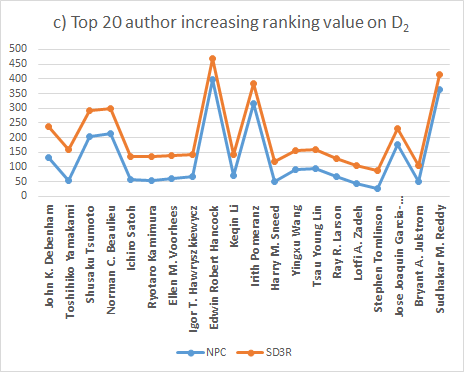
\includegraphics[width=0.45\textwidth]{D2t20ainc}
    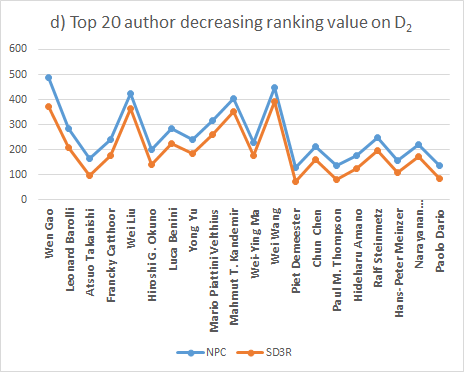
\includegraphics[width=0.45\textwidth]{D2t20adec}
\end{figure}
%
\begin{table}
\begin{center}
\caption{The average $\%\Delta^{NPC,SD4R}$ and the Spearman's rank correlation coefficient of author and conference using NPC, SD4R models on $D_1, D_2$}
\label{fig:deltaresult}
%\caption{default}
{\scriptsize
\begin{tabular}{|c|c|c|c|c|}
\hline
Dataset	& $avg(\%\Delta^{NPC,SD4R}_a)$ & $avg(\%\Delta^{NPC,SD4R}_c)$ & $\rho^{NPC,SD4R}_a$ & $\rho^{NPC,SD4R}_c$ \\
\hline\hline
$D_1$ &	$34.4\%$ & $5.6\%$ & 0.97 & 0.99 \\
$D_2$ & $29.6\%$ & $7.6\%$ & 0.98 & 0.99 \\
\hline
\end{tabular}
}
\end{center}
\end{table}
%
%
\begin{itemize}
\item \textit{SD4R ranking scores reflect how hot the conferences are}. Fig~\ref{Fig:Top20IncDecConference} has show the top 20 conferences most increasing and decreasing the ranking score over $D_2$. All \textit{increasing} conferences are young, annual events and get hot topics now. For example, the top five topics are about remote sensing (IGARSS - IEEE International Geoscience and Remote Sensing Symposium, from 2005), computer human interaction (CHI - Computer Human Interaction, from 1990), medical image computing (MICCAI - Medical Image Computing and Computer - Assisted Intervention, from 1998), (ISBI - IEEE International Symposium on Biomedical Imaging, from 2002), solid-state circuits (ISSCC - International Solid-State Circuits Conference, from 2009)\ldots
On the other hand, the top five \textit{decreasing} conferences are held for over a long time or biennial events, in local community (GI-Jahrestagung - language spoken is Germany, from 1972) or with less interesting topics such as performance evaluation (CMG - Computer Measurement Group Conference, from 1976), artificial intelligence (IJCAI -  International Joint Conference on Artificial Intelligence, biennial from 1969, AAAI - Conference on Artificial Intelligence, from 1980), image processing(IFIP - International Federation for Information Processing, biennial from 1959),\ldots
%

\item\textit{SD4R ranks authors differently and is perfect monotonic with NPC}.
\\
According to Tab.~\ref{fig:deltaresult}, the average of $\%\Delta^{NPC,SD4R}_a$ of conferences is small less than $10\%$, whereas that number of authors is much higher, around $30\%$. It implies that SD4R and NPC methods have similar results in ranking conferences but significantly different results in ranking authors. The Spearman correlation coefficients indicate that the rank results of both methods are perfect monotone. Fig.~\ref{Fig:Top20Author} shows the significantly different in top 20 authors ranking for both methods.
\item\textit{SD4R reflects the contribution of the author betters than the NPC}. Fig.~\ref{Fig:Top20IncDecAuthor} has show the top 20 authors most increasing and decreasing the ranking score over $D_2$. We observe that all top \textit{decreasing} authors are have a large number of publications. Their publications have a large number of co-authors. All top \textit{increasing} authors are really key-person in their research topics.
\end{itemize}
%
\begin{figure} %this figure will be at the right
	\caption{Comparing top 20 authors NPC vs. SD4R over D2, $\alpha_2=0.45$}
	\label{Fig:Top20Author}
    \centering
    \includegraphics[width=0.45\textwidth]{D1t20aNPC}
    \includegraphics[width=0.45\textwidth]{D1t20aSD4R}
    \includegraphics[width=0.45\textwidth]{D2t20aNPC}
    \includegraphics[width=0.45\textwidth]{D2t20aSD4R}
\end{figure}
%

%
\subsubsection{With citation information}
%
%
\begin{itemize}
\item \textit{SC4R rank conferences prestigiously}. Fig.~\ref{Fig:Top20ConferenceD3} shows the significantly different of SC4R model when comparing to H-index, SD4R and NPC models. While NPC and SD4R rank conferences similarly, SC4R can reflect the prestige of conferences better. Except HICSS - Hawaii International Conference on System Sciences having more than ten thousand papers, VLDB - Very Large Data Bases, SIGMOD - International Conference on Management of Data, ICDE - International Conference on Data Engineering and PODS - Symposium on Principles of Database Systems, listing in the top five of SC4R ranking conferences, are very noble in database field following the assessment of experts.

\item\textit{SC4R reflects the contribution of the author betters than others}. Fig~\ref{Fig:Top20AuthorD3} has show the top 20 highest rank value of authors for each method over $D_3$.

%We observe that authors with most cite. Their publications have a large number of co-authors. All top \textit{increasing} authors are really key-person in their research topics.
\end{itemize}
\begin{figure} %this figure will be at the right
	\caption{Top 20 ranking value of conference by NPC, SD4R, H-index and SC4R on $D_3$ with $\alpha_1=0.3$}
	\label{Fig:Top20ConferenceD3}
    \centering
    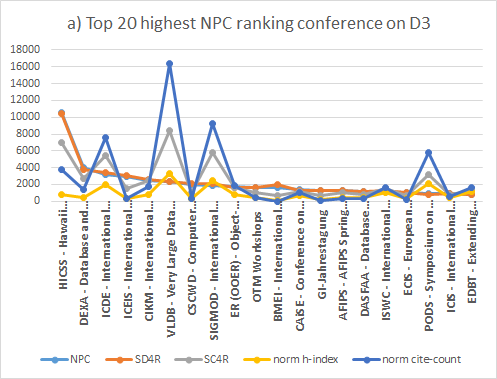
\includegraphics[width=0.45\textwidth]{D3t20cNPC}
    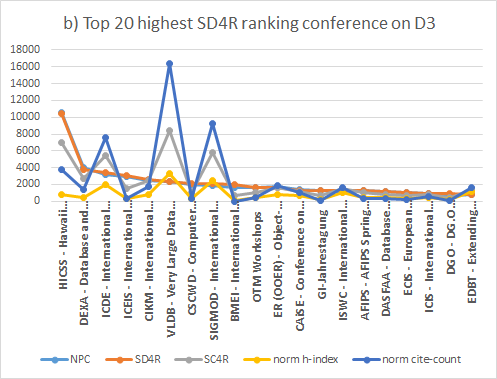
\includegraphics[width=0.45\textwidth]{D3t20cSD4R}

    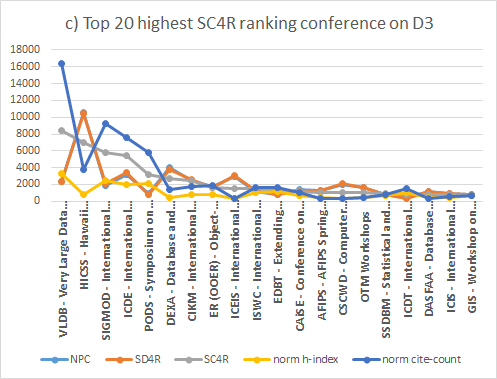
\includegraphics[width=0.45\textwidth]{D3t20cSC4R}
    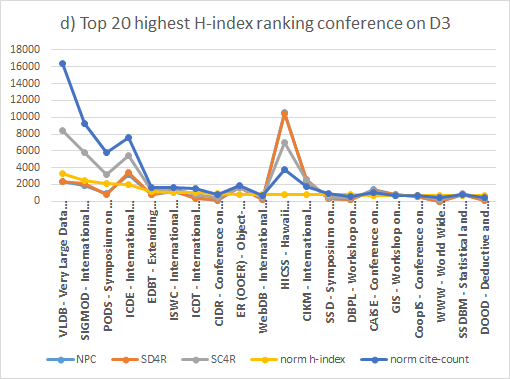
\includegraphics[width=0.45\textwidth]{D3t20cHindex}
\end{figure}

\begin{figure} %this figure will be at the right
	\caption{Top 20 ranking value of author by NPC, SD4R, H-index and SC4R on $D_3$ with $\alpha_1=0.3$}
	\label{Fig:Top20AuthorD3}
    \centering
    \includegraphics[width=0.45\textwidth]{D3t20aNPCh}
    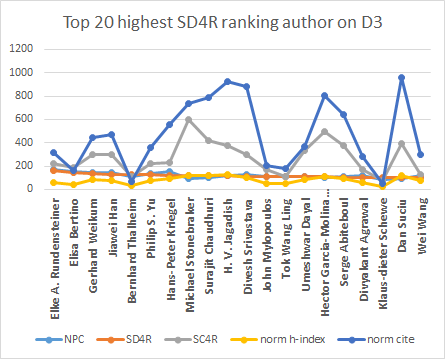
\includegraphics[width=0.45\textwidth]{D3t20aSD4Rh}
     \includegraphics[width=0.45\textwidth]{D3t20aHindex}
     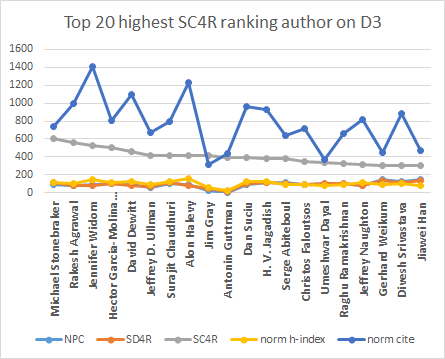
\includegraphics[width=0.45\textwidth]{D3t20aSC4Rh}
\end{figure}

\section{Related work}\label{Sect:Related}
\textit{Our prior work}. Our work is the extend version of the prior work \cite{Vu14}. In this version, we has extend the experiments and represent everything more in detail. Concretely, we do the experiments for the case the citations are considered. We also compare our ranking with the H-index, which is the most famous ranking scores for authors recently. Moreover, we improve the results by giving more discussions.

The ranking problem occurs and develop quickly with the era of the Internet and big data. One of the most famous ranking problem is ranking web-pages. A brief overview of this problem can be found at Dilip Kumar Sharma et al. \cite{RankOverview}. PageRank were utilized by Google search engine \cite{pagerank98}.
Since the hyperlink structure among the web-pages are easily represented as a web graph,
the PageRank of each web-page can be measured (see Sect.~\ref{Sect:PageRank} for more detail). Hyperlink-Induced Topic Search (HITS) is a link analysis algorithm that rates Web pages, developed by Jon Kleinberg \cite{HIndex}. It was a precursor to PageRank. The idea behind HITS algorithm classify the webs into two classes: (i) hubs, served as large directories point to (ii) authoritative pages. A good hub represented a page that pointed to many other pages, and a good authority represented a page that was linked by many different hubs. The model can be rewritten into 2-linear ranking model.

\textit{Named entities:}
In Natural Language Processing (NLP) communities, named entity recognition is an important problem.
Ranking scheme has been applied to solve the problem. Collins \cite{Collins-ACL-02} proposes a ranking method based on a maximum-entropy tagger. Also,
Vercoustre et al. \cite{Vercoustre-SAC-08} has presented how to apply the ranking method to Wikipedia.

\textit{Scientific articles}
In bibliometrics, the scientific articles (e.g., research papers, technical reports, and so on) are evaluated with respect to the quality (e.g., novelty and originality) as well as academic influence to the communities (e.g., impact) by relaying on the citations (e.g., references and quotation) \cite{Cronin-JIS-01}.

\textit{Researchers}
Also, Researchers has been ranked by citation analysis (e.g., how many papers has he/she published, how many times have his/her papers cited, and so on). More interestingly, H-index (Hirsch index) has been designed to
measure both the productivity and impact of the published work of the researchers.

\textit{Complex system}
The complex system ranking has been already explored using a different formalism for ranking or classification in heterogeneous networks \cite{poprank,complexrank}.
The poprank model \cite{poprank} introduce the Popularity Propagation Factor to express the relationship between classes. Their model is based on the markov chain model which can be applied in the N-linear mutual ranking systems. The quantium ranking \cite{complexrank} is based on quantium navigation. Their formula is come from the quantium theory and quite different to ours.

So far, conferences have been ranked by subjective opinions and consensus among well known experts in a domain.
Such lists in computer science area are compiled here\footnote{http://intelligent.pe.kr/ConfRank.txt}.
In this work, we have proposed a novel conference ranking framework to integrate all possible evidence.



%%%%%%%%%%%%%%%%%%%%%%%%%%%%%%%%%%%%%%%%%%%%%%%%%%%%%%%%%%%%%%%%%%
\section{Conclusion and future works}\label{Sect:Conclusion}
We have introduced and studied N-star ranking for mutual ranking systems. The mutual relationships between ranking objects are described by a system of linear equations, N-mutual ranking system. A N-linear mutual ranking system is a N-star ranking systems if it has a core class which affects and reflects all other classes in the system. The rank scores of the N-star ranking system are unique and computed by a Markov chain. We have pointed out that PageRank is a 2-star ranking. It has two classes:  the web-pages (a core class) and links.

We have introduced and studied a general and a simple 4-star ranking models for ranking authors, publications, conferences. A general model is a generic one. In a simple model, we consider each publication, author, conference, citation is equally. We have conducted the experiments for the models in which the citations are not considered. The experimental results are based on the DBLP dataset. By comparing the difference between the SD4R vs. NPC models, we have shown that our ranking system can reflect how hot the conference are and record the contribution of the authors better than the naive ranking system. Moreover, our ranking system makes a big change on author ranking.

As future work, we are planning to $i$) get the citations between the publication to upgrade the quality of our ranking system, $ii$) study how to combine a N-star ranking systems with a given ranking systems, $iii$) investigate the time series in N-star ranking and the trend prediction problem, and $iv$) apply N-star ranking systems in various ranking problems, e.g., business ranking, event ranking, and so on.

\vspace{-3ex}
\begin{thebibliography}{99}
\setlength{\parskip}{-3pt}\vspace{-2ex}

\bibitem{Vercoustre-SAC-08}
\textbf{Anne-Marie Vercoustre, James A. Thom, Jovan Pehcevski.}
Entity ranking in Wikipedia.
\textit{Proceedings of the 2008 ACM symposium on Applied computing (SAC'08)},
(2008) 1101-1106.

\bibitem{HIndex06}
\textbf{A. Sidiropoulos, D. Katsaros, Y. Manolopoulos.}
Generalized Hirsch h-index for disclosing latent facts in citation networks.
\textit{Scientometrics,} \textbf{Vol. 72 (2)}, (2006) 253--280.

\bibitem{Cronin-JIS-01}
\textbf{Blaise Cronin.}
Bibliometrics and beyond: some thoughts on web-based citation analysis.
\textit{Journal of Information Science},
\textbf{Vol. 27 (1)}, (2001), 1--7 .


\bibitem{Markov11}
\textbf{C. Freudenthaler, S. Rendle and L. S. Thieme.}
Factorizing Markov Models for Categorical Time Series Prediction.
\textit{In Proceedings of ICNAAM, } (2011) 405-409.

\bibitem{complexrank}
\textbf{Eduardo Sánchez-Burillo, Jordi Duch, Jesús Gómez-Gardenes, David Zueco.}
Quantum Navigation and Ranking in Complex Networks
\textit{Nature online journal} (2012).

\bibitem{HIndex}
\textbf{J. E. Hirsch}
An index to quantify an individual's scientific research output.
\textit{Proceedings of the National Academy of Sciences of the United States of America} \textbf{102(46)}
(2005), 16569–-16572.



\bibitem{Keener1993}
\textbf{J. Keener.}
The Perron-Frobenius theorem and the ranking of football teams.
\textit{SIAM Review}, \textbf{Vol. 35(1)}, (1993), 80--93.

\bibitem{HITS}
\textbf{Jon Kleinberg}
Authoritative Sources in a Hyperlinked Environment.
\textit{Journal of the ACM}, \textbf{Vol. 46 (5)}, (1999), 604-632.



\bibitem{Kien09}
\textbf{L. T. Kien, L. T. Hieu, T. L. Hung, L. A. Vu.}
MpageRank: The Stability of Web Graph.
\textit{Vietnam Journal of Mathematics}, \textbf{Vol. 37}, (2009), 475--489

\bibitem{Collins-ACL-02}
\textbf{Michael Collins.}
Ranking algorithms for named-entity extraction: boosting and the voted perceptron.
\textit{Proceedings of the 40th Annual Meeting on Association for Computational Linguistics,}
(2002), 489--496.


\bibitem{MichaelLey09}
\textbf{Michael Ley.}
DBLP - Some Lessons Learned.
\textit{PVLDB} 2 (2), (2009) 1493--1500.



\bibitem{MichaelLey06}
\textbf{Michael Ley, Patrick Reuther.}
Maintaining an Online Bibliographical Database: The Problem of Data Quality.
\textit{EGC 2006}, (2006) 5--10.




\bibitem{microsoft}
\textbf{Microsoft  Corporation.}
Microsoft Academic Search.
\textit{http://academic.research.microsoft.com/} (June -26 -2013).



\bibitem{pagerank98}
\textbf{S. Brin and L. Page.}
The anatomy of a large-scale hypertextual web search engine.
\textit{In Proceedings of the 7th International World Wide Web
Conference}, (1998), 107--117



\bibitem{MarkovWWW10}
\textbf{S. Rendle, C. Freudenthaler, L. S. Thieme.}
Factorizing personalized Markov chains for next-basket recommendation.
\textit{Proceedings of the 19th international conference on World wide web}, (2010) 811--820.

\bibitem{RankOverview}
\textbf{Sharma, Dilip Kumar and Sharma A. K}
A comparative analysis of web page ranking algorithms.
\textit{International Journal on Computer Science and Engineering} . (2010) 2670--2676.

\bibitem{Markov10}
\textbf{T. Furukawa, S. Okamoto, Y. Matsuo, M. Ishizuka.}
Prediction of social bookmarking based on a behavior transition model.
\textit{Proceedings of the 2010 ACM Symposium on Applied Computing}, (2010) 1741--1747.

\bibitem{Vu14}
\textbf{Vu, L. A., Hai, V. H., Hieu, L. T., Kien, L. T.  and Jason, J. J. }
A General Model for Mutual Ranking Systems,
\textit{Intelligent Information and Database Systems
Lecture Notes in Computer Science}, \textbf{8397} (2014), 211--200.


\bibitem{poprank}
\textbf{Z. Nie and Y. Zhang and J. Wen and W. Ma.}
Object-Level Ranking: Bringing Order to Web Objects,
Study of the eXplicit Control Protocol (XCP).
\textit{IEEE Infocom }(2005).


\end{thebibliography}
\vspace{2cm}

\noindent\textbf{Vu Le Anh}\\
Nguyen Tat Thanh University\\
Ho Chi Minh City\\
Vietnam\\
{\tt e-mail lavu@ntt.edu.vn}\\

\noindent\textbf{Vo Hoang Hai}\\
Information Technology College\\
Ho Chi Minh city\\
Vietnam\\
{\tt e-mail vohoanghai2@gmail.com}\\

\noindent\textbf{Hieu Le Trung}\\
Duy Tan University\\
Da Nang\\
Vietnam\\
{\tt e-mail hieukien82@gmail.com}\\

\noindent\textbf{Kien Le Trung}\\
University of Science\\
Thua Thien Hue\\
Vietnam\\
{\tt e-mail hieukien@hotmail.com}\\

\noindent\textbf{Jason J. Jung}\\
Yeungnam University\\
Gyeongsan\\
Korea\\
{\tt e-mail }

\end{document}
